\pagebreak
\section{Direct Memory Access (DMA)}
Usando ADC e USART per fare misure e trasferire dati, una delle più grandi limitazioni in velocità è il tempo di trasferimento dei dati dalla periferica al microcontrollore. Questo tempo è dovuto al fatto che la CPU deve leggere i dati dalla periferica e salvarli in memoria.\\

\subsection{Funzionamento}

Il processo per trasferire dati dalla periferica alla memoria presume che il dato, prima di essere salvato nella memoria RAM, sia salvato nella memoria interna alla CPU in modo che la CPU ci possa lavorare. \\
Questo passaggio si può rimuovere usando il DMA.

\begin{figure}[h]
    \centering
    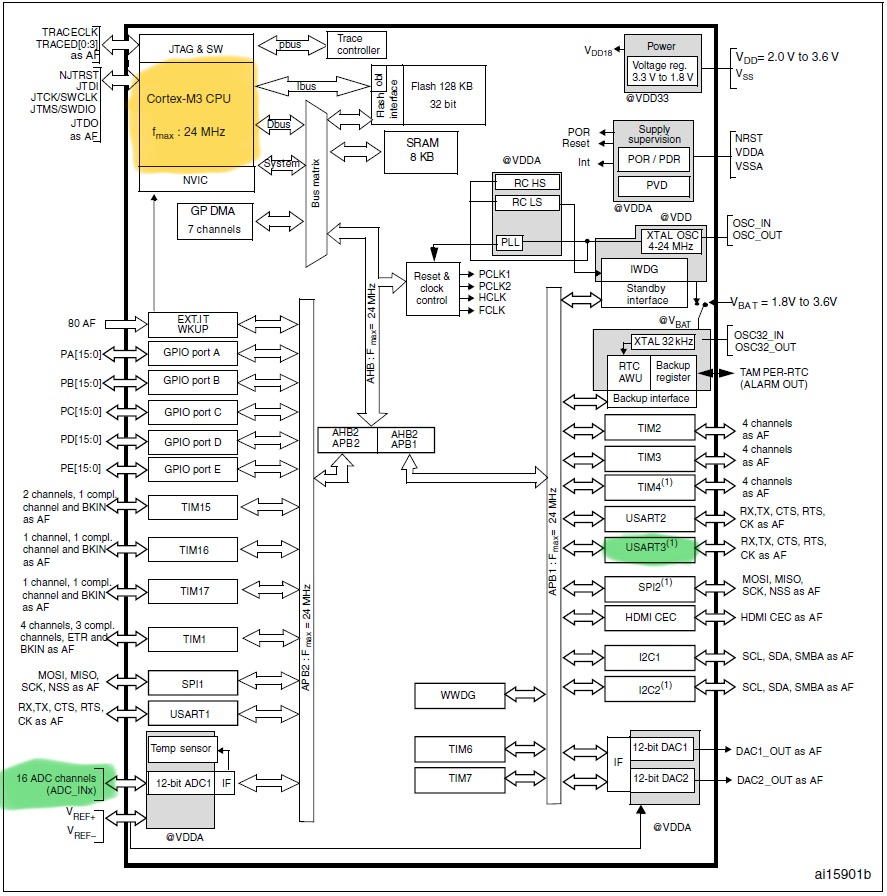
\includegraphics[width=0.8\linewidth]{microcontrollore/assets/Cortex_structure.jpg}
    \caption{Struttura interna del microcontrollore}
    \label{fig:Cortex}
\end{figure}

Una volta configurato, il DMA permette di evitare il carico computazionale della CPU per il trasferimento dei dati dando l'accesso diretto alla periferica di accedere alla memoria.
Così facendo, oltre alla CPU più libera, i dati saranno salvati direttamente dalle periferiche nella memoria nella maniera più veloce possibile.\\

\subsection{Programmazione}
Dato che il protocollo del DMA ti permette di salvare i dati in autonomia, la parte di programmazione consiste solo nel configurare correttamente il DMA.\\



Dato che può essere molto complesso, parte della configurazione è stata fatta con il code generator di STM32CubeIDE e consiste nel collegare uno \textit{stream} del DMA alla periferica che si vuole usare e dargli la dimensione del dato e in che tipo di memoria si vuole salvare.\\

\begin{wrapfigure}{r}{0.4\linewidth}
    \centering
    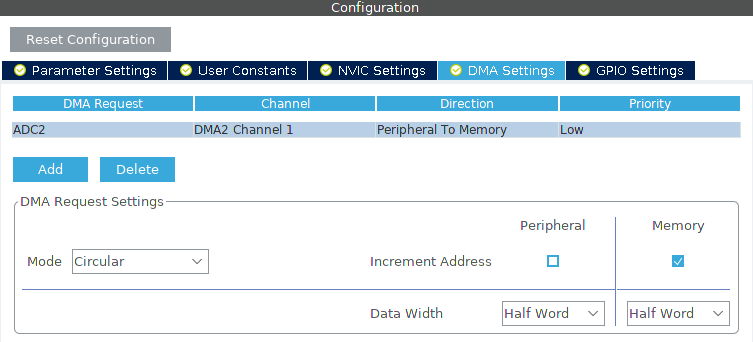
\includegraphics[width=\linewidth]{microcontrollore/assets/dma_configuration.png}
    \caption{Configurazione del DMA}
    \label{fig:DMA}
\end{wrapfigure}

Una volta configurato su STM32CubeMX, c'è bisogno di configurare specificatamente il DMA per la periferica che si vuole usare e aggiungere alla periferica l'istruzione che permette di essere collegata al DMA.\\

In generale, questo tipo di configurazione può essere riassunta in 4 righe di codice. Usiamo come esempio il DMA per l'ADC:

\begin{minted}[bgcolor = coding, linenos]{C}
    DMA1_Stream0 -> PAR = (uint32_t) &ADC3->DR; //Collegare il DMA al registro
                                                //che contiene il dato
    DMA1_Stream0 -> M0AR = (uint32_t) &vec_dati; //Dare al DMA l'indirizzo della memoria
                                                //in cui salvare il dato
    DMA1_Stream0 -> NDTR = len; // Dimensione del dato
    ADC3 -> CFGR |=(3<<ADC_CFGR_DMNGT_Pos); // Configura l'ADC per usare il DMA
\end{minted}

e poi si attiva il DMA con la funzione:

\begin{minted}[bgcolor = coding, linenos]{C}
    DMA1_Stream0->CR |= DMA_SxCR_EN // Attiva il DMA
\end{minted}

\begin{flushleft}

    \colorbox{notebox}{
    \begin{minipage}[]{\textwidth}
        Notiamo come, anche se il DMA è attivo, ciò non va a modificare il funzionamento degli interrupt. Anche se il DMA controlla il flusso dei dati, noi possiamo comunque accedere a qualsiasi dato (misurato o trasmesso) in qualsiasi momento.
    \end{minipage}
    }
\end{flushleft}